\documentclass[border=0.2cm]{standalone}
\usepackage{tikz}
\usepackage{titlesec}
\usepackage{float}
\usepackage{standalone}
\usepackage{tikzit}
\usetikzlibrary{automata, arrows.meta, positioning}
\usetikzlibrary{arrows.meta, positioning}
\input{sample-02.tikzstyles}

\begin{document}
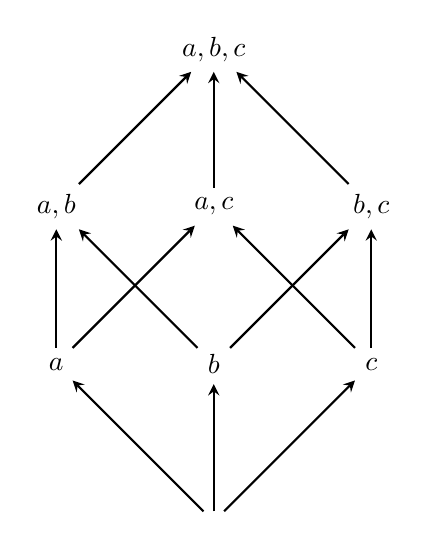
\begin{tikzpicture}[->, >=stealth, thick]
\node (1) at (4,0) {$\varnothing$};
\node (2) at (2,2) {$\set{a}$};
\node (3) at (4,2) {$\set{b}$};
\node (5) at (6,2) {$\set{c}$};
\node (6) at (2,4) {$\set{a, b}$};
\node (10) at (4,4) {$\set{a, c}$};
\node (15) at (6,4) {$\set{b, c}$};
\node (30) at (4,6) {$\set{a, b, c}$};
\draw (1) -- (2);
\draw (1) -- (3);
\draw (1) -- (5);
\draw (2) -- (6);
\draw (2) -- (10);
\draw (3) -- (6);
\draw (3) -- (15);
\draw (5) -- (10);
\draw (5) -- (15);
\draw (6) -- (30);
\draw (10) -- (30);
\draw (15) -- (30);
\end{tikzpicture}
\end{document}
